\section{Defining the Simulation}

The parameters for PyLith are specified as a hierarchy or tree of
modules. The application assembles the hierarchy of modules from user
input and then calls the \object{main} function in the top-level
module in the same manner as a C or C++ program. The behavior of the
application is determined by the modules included in the hierarchy as
specified by the user. The Pyre framework provides the interface for
defining this hierarchy. Pyre properties correspond to simple settings
in the form of strings, integers, and real numbers. Pyre facilities
correspond to software modules. Facilities may have their own
facilities (branches in the tree) and any number of properties. See
Figure \vref{fig:Pyre:Architecture} for the general concept of Pyre
facilities and properties. The top-level object is the PyLith
application with three facilities: \facility{mesher}, \facility{problem},
and \facility{petsc}. The \facility{mesher} specifies how to import the
mesh, the \facility{problem} specifies the physical properties, boundary
conditions, etc., and \facility{petsc} is used to specify PETSc
settings. Appendix \vref{cha:components} contains a list of the
components provided by PyLith and spatialdata.


\subsection{Setting PyLith Parameters}
\label{sec:setting:parameters}

There are several methods for setting input parameters for the
\filename{pylith} executable: via the command line or by using a text
file in \filename{.cfg} or \filename{.pml} format. Both facilities and
properties have default values provided, so you only need to set
values when you want to deviate from the default behavior.


\subsubsection{Units}

All dimensional parameters require units. The units are specified
using Python and FORTRAN syntax, so square meters is m**2. Whitespace
is not allowed in the string, for units and dimensioned quantities
are multiplied by the units string; for example, two meters per second
is 2.0*m/s. Available units are shown in Table \vref{tab:pyre:units}

\begin{table}[htbp]
\caption{Pyre supported units. Aliases are in parentheses.}
\label{tab:pyre:units}
\begin{tabular}{lp{5in}}
\textbf{Scale} & \textbf{Available Units} \\
\hline 
length & meter (m), micrometer (um, micron), millimeter (mm), centimeter (cm),
kilometer (km), inch, foot, yard, mile \\
time & second (s), nanosecond (ns), microsecond (us), millisecond (ms), minute,
hour, day, year \\
mass & kilogram (kg), gram (g), centigram (cg), milligram (mg), ounce, pound,
ton \\
pressure & pascal (Pa), kPa, MPa, GPa, bar, millibar, atmosphere (atm) \\
\hline 
\end{tabular}
\end{table}


\subsubsection{Using the Command Line}

The \commandline{-}-help} command line argument displays links to useful
resources for learning PyLith.

Pyre uses the following syntax to change properties from the command
line. To change the value of a property of a component, use
\commandline{-{}-COMPONENT.PROPERTY=VALUE}. Each component is attached
to a facility, so the option above can also be written as
\commandline{-{}-FACILITY.PROPERTY=VALUE}.  Each facility has a
default component attached to it. A different component can be
attached to a facility by \commandline{-{}-FACILITY=NEW\_COMPONENT}.

PyLith's command-line arguments can control Pyre and PyLith properties
and facilities, MPI settings, and PETSc settings. All PyLith-related
properties are associated with the \facility{pylithapp} component. You
can get a list of all of these top-level properties along with a
description of what they do by running PyLith with the
\commandline{-{}-help-properties} command-line argument. To get
information on user-configurable facilities and components, you can
run PyLith with the \commandline{-{}-help-components} command-line
argument. To find out about the properties associated with a given
component, you can run PyLith with the
\commandline{-{}-COMPONENT.help-properties} flag:
\begin{shell}
$$ pylith --problem.help-properties
# Show problem components.
$$ pylith --problem.help-components
# Show bc components (bc is a component of problem).
$$ pylith --problem.bc.help-components
# Show bc properties.
$$ pylith --problem.bc.help-properties
\end{shell}


\subsubsection{Using a {\ttfamily .cfg} File}

Entering all those parameters via the command line involves the risk
of typographical errors. You
will generally find it easier to collect parameters into a
\filename{.cfg} file. The file is composed of one or more sections
which are formatted as follows:
\begin{cfg}
<h>[pylithapp.COMPONENT1.COMPONENT2]</h>
# This is a comment.

<f>FACILITY3</f> = COMPONENT3
<p>PROPERTY1</p> = VALUE1
<p>PROPERTY2</p> = VALUE2 ; this is another comment
\end{cfg}

\tip{We strongly recommend that you use \filename{.cfg} files for your
  work.  The files are syntax-highlighted in the vim editor.}


\subsubsection{Using a {\ttfamily.pml} File}

A \filename{.pml} file is an XML file that specifies parameter values
in a highly structured format. It is composed of nested sections which
are formatted as follows:
\begin{lstlisting}[basicstyle=\ttfamily,frame=tb]{language=xml}
<component~name="COMPONENT1">
    <component~name="COMPONENT2">
        <property~name="PROPERTY1">VALUE1</property>
        <property~name="PROPERTY2">VALUE2</property>
    </component>
</component>
\end{lstlisting}
XML files are intended to be read and written by machines, not edited
manually by humans. The \filename{.pml} file format is intended for
applications in which PyLith input files are generated by another
program, e.g., a GUI, web application, or a high-level structured
editor. This file format will not be discussed further here, but if
you are interested in using \filename{.pml} files, note that \filename{.pml}
files and \filename{.cfg} files can be used interchangeably; in the
following discussion, a file with a \filename{.pml} extension can be
substituted anywhere a \filename{.cfg} file can be used.


\subsubsection{Specification and Placement of Configuration Files}

Configuration files may be specified on the command line:
\begin{shell}
$$ pylith example.cfg
\end{shell}
In addition, the Pyre framework searches for configuration files named
\filename{pylithapp.cfg} in several predefined locations. You may put
settings in any or all of these locations, depending on the scope
you want the settings to have:
\begin{enumerate}
\item \filename{\$PREFIX/etc/pylithapp.cfg}, for system-wide settings;
\item \filename{\$HOME/.pyre/pylithapp/pylithapp.cfg}, for user
  settings and preferences;
\item the current directory (\filename{./pylithapp.cfg}), for local
  overrides.
\end{enumerate}

\important{The Pyre framework will search these directories for
  \filename{.cfg} files matching the names of components (for example,
  \filename{timedependent.cfg}, \filename{faultcohesivekin.cfg},
  \filename{greensfns.cfg}, \filename{pointforce.cfg}, etc) and will
  attempt to assign all parameters in those files to the respective
  component.}

\important{Parameters given directly on the command line will override
  any input contained in a configuration file. Configuration files
  given on the command line override all others. The
  \filename{pylithapp.cfg} files placed in (3) will override those in
  (2), (2) overrides (1), and (1) overrides only the built-in
  defaults.}

All of the example problems are set up using configuration files and specific problems are defined by including
the appropriate configuration file on the command-line. Referring
to the directory \filename{examples/twocells/twohex8}, we have the
following.
\begin{shell}
$$ ls -1 *.cfg
axialdisp.cfg
dislocation.cfg
pylithapp.cfg
sheardisp.cfg
\end{shell}
The settings in \filename{pylithapp.cfg} will be read automatically, and additional
settings are included by specifying one of the other files on the
command-line:
\begin{shell}
$$ pylith axialdisp.cfg
\end{shell}
If you want to see what settings are being used, you can either examine
the \filename{.cfg} files, or use the help flags as described above:
\begin{shell}
# Show components for the 'problem' facility.
$$ pylith axialdisp.cfg --problem.help-components
# Show properties for the 'problem' facility.
$$ pylith axialdisp.cfg --problem.help-properties
# Show components for the 'bc' facility.
$$ pylith axialdisp.cfg --problem.bc.help-components
# Show properties for the 'bc' facility.
$$ pylith axialdisp.cfg --problem.bc.help-properties
\end{shell}
This is generally a more useful way of determining problem settings,
since it includes default values as well as those that have been specified
in the \filename{.cfg} file.


\subsubsection{List of PyLith Parameters ({\ttfamily pylithinfo})}
\label{sec:pylithinfo}

The Python application \filename{pylithinfo} writes all of the current
parameters to a text file or JSON file (default). The default name of the JSON is \filename{pylith\_parameters.json}.
The usage synopsis is
\begin{shell}
$$ pylithinfo [--verbose-false] [--format={ascii,json} [--filename=pylith_parameters.json] PYLITH_ARGS
\end{shell}
where \commandline{-{}-verbose-false} turns off printing the descriptions of
the properties and components as well as the location where the
current value was set, \commandline{-{}-format=ascii} changes the
output format to a simple ASCII file, and
\commandline{-{}-filename=pylith\_parameters.json} sets the name of the
output file. The PyLith Parameter Viewer (see Section
\ref{sec:pylith:parameter:viewer}) provides a graphic user interface
for examining the JSON parameter file. 


\subsection{Mesh Information (\ttfamily{mesher})}

Geometrical and topological information for the finite element mesh
may be provided by exporting an Exodus II format file from
CUBIT/Trelis, by exporting a GMV file and an accompanying Pset file
from LaGriT, or by specifying the information in PyLith mesh ASCII
format. See Chapter \vref{cha:examples} for examples.

PyLith supports linear cells in 2D (Figure \vref{fig:2D:cells}), and
3D (Figure \vref{fig:3D:cells}).  The vertex ordering must follow the
convention shown in Figures \vref{fig:2D:cells}-\vref{fig:3D:cells}.
PyLith no longer supports use of quadratic cells using the PyLith
ASCII mesh format. In the next release, we plan to support higher
order discretizations via PETSc finite-element features from meshes
with linear cells as input.

The mesh information defines the vertex coordinates and specifies
the vertices composing each cell in the mesh. The mesh information
must also define at least one set of vertices for which displacement
(Dirichlet) boundary conditions will be provided. In most realistic
problems, there will be several vertex groups, each with a unique
identifying label. For example, one group might define a surface of
the mesh where displacement (Dirichlet) boundary conditions will be
applied, another might define a surface where traction (Neumann) boundary
conditions will be applied, while a third might specify a surface
that defines a fault. Similarly, the mesh information contains cell
labels that define the material type for each cell in the mesh. For
a mesh with a single material type, there will only be a single label
for every cell in the mesh. See Chapters \vref{cha:material:models}
and \vref{cha:boundary:interface:conditions} for more detailed discussions
of setting the materials and boundary conditions.

\begin{figure}[htbp]
  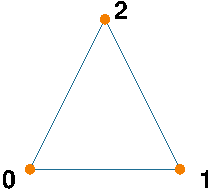
\includegraphics{runpylith/figs/tri3}\hspace*{0.5in}%
  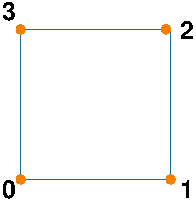
\includegraphics{runpylith/figs/quad4}
  \caption{Linear cells available for 2D problems are the triangle
    (left) and the quadrilateral (right).}
  \label{fig:2D:cells}
\end{figure}

\begin{figure}[htbp]
  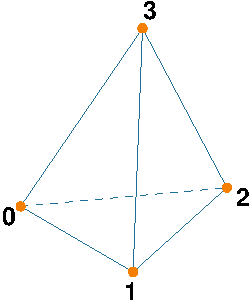
\includegraphics{runpylith/figs/tet4}\hspace*{0.5in}%
  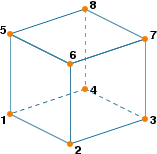
\includegraphics{runpylith/figs/hex8}
  \caption{Linear cells available for 3D problems are the tetrahedron (left)
    and the hexahedron (right).}
  \label{fig:3D:cells}
\end{figure}

\subsubsection{\object{Mesh Importer}}

The default mesher component is \object{MeshImporter}, which provides
the capabilities of reading the mesh from files. The \object{MeshImporter} has
several properties and facilities:
\begin{inventory}
  \propertyitem{reorder\_mesh}{Reorder the vertices and cells using the
    reverse Cuthill-McKee algorithm (default is False)}
  \facilityitem{reader}{Reader for a given type of mesh (default is
    \object{MeshIOAscii}).}
  \facilityitem{distributor}{Handles
    distribution of the mesh among processors.}
  \facilityitem{refiner}{Perform global uniform mesh refinement after
    distribution among processors (default is no refinement).}
\end{inventory}
Reordering the mesh so that vertices and cells connected topologically
also reside close together in memory improves overall performance
and can improve solver performance as well.

\warning{The coordinate system associated with the mesh must be a
  Cartesian coordinate system, such as a generic Cartesian coordinate
  system or a geographic projection.}

\subsubsection{\object{MeshIOAscii}}

The \object{MeshIOAscii} object is intended for reading small, simple
ASCII files containing a mesh constructed by hand. We use this file
format extensively in the examples. Appendix \vref{sec:format:MeshIOAscii}
describes the format of the files. The properties and facilities of
the \object{MeshIOAscii} object include:
\begin{inventory}
\propertyitem{filename}{Name of the mesh file.}
\facilityitem{coordsys}{Coordinate system associated with the mesh.}
\end{inventory}

\subsubsection{\object{MeshIOCubit}}
\label{sec:MeshIOCubit}

The \object{MeshIOCubit} object reads the NetCDF Exodus II files output from
CUBIT/Trelis. Beginning with CUBIT 11.0, the names of the nodesets are included
in the Exodus II files and PyLith can use these nodeset names or revert
to using the nodeset ids. The properties and facilities associated
with the \object{MeshIOCubit} object are:
\begin{inventory}
\propertyitem{filename}{Name of the Exodus II file.}
\propertyitem{use\_nodeset\_names}{Identify nodesets by name rather than id
(default is True).}
\facilityitem{coordsys}{Coordinate system associated with the mesh.}
\end{inventory}

\subsubsection{\object{MeshIOLagrit}}
\label{sec:MeshIOLagrit}

The \object{MeshIOLagrit} object is used to read ASCII and binary GMV and PSET
files output from LaGriT. PyLith will automatically detect whether
the files are ASCII or binary. We attempt to provide support for experimental
64-bit versions of LaGriT via flags indicating whether the FORTRAN
code is using 32-bit or 64-bit integers. The \object{MeshIOLagrit} properties
and facilities are:
\begin{inventory}
  \propertyitem{filename\_gmv}{Name of GMV file.}
  \propertyitem{filename\_pset}{Name of the PSET file.}
  \propertyitem{flip\_endian}{Flip the endian of values when reading
    binary files (default is False).}
  \propertyitem{io\_int32}{Flag
    indicating that PSET files use 32-bit integers (default is True).}
  \propertyitem{record\_header\_32bt}{Flag indicating FORTRAN record header is
    32-bit (default is True).}
\facilityitem{coordsys}{Coordinate system associated with mesh.}
\end{inventory}

\warning{The PyLith developers have not used LaGriT since around 2008
  and the most recent release appears to have been in 2010.}

\subsubsection{\object{Distributor}}

The distributor uses a partitioner to compute which cells should be
placed on each processor, computes the overlap among the processors,
and then distributes the mesh among the processors. The type of
partitioner is set via PETSc settings. The properties and facilities
of the \object{Distributor} include:
\begin{inventory}
\propertyitem{partitioner}{Name of mesh partitioner ['chaco','parmetis'].}
\propertyitem{write\_partition}{Flag indicating that the partition information
should be written to a file (default is False).}
\facilityitem{data\_writer}{Writer for partition information (default
  is \object{DataWriterVTK} for VTK output).}
\end{inventory}
An example of setting the partitioner in a \filename{pylithapp.cfg}
  file is:
\begin{cfg}
<h>[pylithapp.mesh_generator.distributor]</h>
<p>partitioner</p> = chaco ; Options are 'chaco' (default) and 'parmetis'.
\end{cfg}
METIS/ParMETIS are not included in the PyLith binaries due to licensing
issues. 


\subsubsection{\object{Refiner}}

The refiner is used to decrease node spacing by a power of two by
recursively subdividing each cell by a factor of two. In a 2D triangular
mesh a node is inserted at the midpoint of each edge, splitting each
cell into four cells (see Figure \vref{fig:uniform:refinement:2x}).
In a 2D quadrilateral mesh a node is inserted at the midpoint of each
edge and at the centroid of the cell, splitting each cell into four
cells. In a 3D tetrahedral mesh a node is inserted at the midpoint
of each edge, splitting each cell into eight cells. In a 3D hexahedral
mesh a node is inserted at the midpoint of each edge, the centroid
of each face, and at the centroid of the cell, splitting each cell
into eight cells.

\begin{figure}[htbp]
  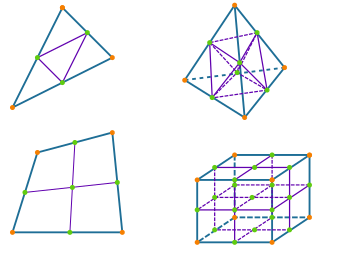
\includegraphics[scale=1.25]{runpylith/figs/refinement2x}
  \caption{Global uniform mesh refinement of 2D and 3D linear
    cells. The blue lines and orange circles identify the edges and
    vertices in the original cells. The purple lines and green circles
    identify the new edges and vertices added to the original cells to
    refine the mesh by a factor of two.}
\label{fig:uniform:refinement:2x}
\end{figure}

Refinement occurs after distribution of the mesh among processors.
This allows one to run much larger simulations by (1) permitting the
mesh generator to construct a mesh with a node spacing largeer than
that needed in the simulation and (2) operations performed in serial
during the simulation setup phase, such as, adjusting the topology
to insert cohesive cells and distribution of the mesh among processors
uses this much smaller coarse mesh. For 2D problems the global mesh
refinement increases the maximum problem size by a factor of $4^{n}$,
and for 3D problems it increases the maximum problem size by a factor
of $8^{n}$, where $n$ is the number of recursive refinement levels.
For a tetrahedral mesh, the element quality decreases with refinement
so $n$ should be limited to 1-2.


\subsection{Problem Specification (\facility{problem})}

The problem component specifies the basic parameters of the simulation,
including the physical properties, the boundary conditions, and interface
conditions (faults). The current release of PyLith contains two types
of problems, \object{TimeDependent} for use in static, quasi-static,
and dynamic simulations and \object{GreensFns} for computing static
Green's functions. The general properties facilities include:
\begin{inventory}
  \propertyitem{dimension}{Spatial dimension of problem space.}
  \facilityitem{normalizer}{Scales used to nondimensionalize the
    problem (default is \object{NondimElasticQuasistatic}).}
  \facilityitem{materials}{Array of materials comprising the domain
    (default is [material]).}
  \facilityitem{bc}{Array of boundary conditions (default is none).}
  \facilityitem{interfaces}{Array of interface conditions, i.e., faults
    (default is none).}
  \facilityitem{gravity\_field}{Gravity field used to construct body
    forces (default is none).}
  \facilityitem{progress\_ monitor}{Show progress of running
    simulation.}
\end{inventory}
An example of setting these parameters in a \filename{.cfg} file for
a problem is:
\begin{cfg}
<h>[pylithapp.timedependent]</h>
<p>dimension</p> = 3
<f>normalizer</f> = spatialdata.units.NondimElasticQuasistatic
<f>materials</f> = [elastic, viscoelastic]
<f>bc</f> = [boundary_east, boundary_bottom, boundary_west]
<f>interfaces</f> = [SanAndreas, SanJacinto]
<f>gravity_field</f> = spatialdata.spatialdb.GravityField
\end{cfg}

\subsubsection{Nondimensionalization (\facility{normalizer})}

PyLith nondimensionalizes all parameters provided by the user so that
the simulation solves the equations using nondimensional quantities.
This permits application of PyLith to problems across a vast range
of spatial and temporal scales. The scales used to nondimensionalize
the problem are length, pressure, density, and time. PyLith provides
two normalizer objects to make it easy to provide reasonable scales
for the nondimensionalization. The \object{NondimElasticQuasistatic}
normalizer (which is the default) has the following properties:
\begin{inventory}
  \propertyitem{length\_scale}{Distance to nondimensionalize length
    (default is 1.0 km).}
  \propertyitem{shear\_modulus}{Shear modulus to nondimensionalize
    pressure (default is 3.0e+10 Pa).}
  \propertyitem{relaxation\_time}{Relaxation time to
    nondimensionalize time (default is 1.0 year).}
\end{inventory}
An example of setting these parameters in a \filename{.cfg} file for
a problem is:
\begin{cfg}
<h>[pylithapp.timedependent.normalizer]</h>
<p>length_scale</p> = 1.0*km
<p>shear_modulus</p> = 3.0e+10*Pa
<p>relaxation_time</p> = 1.0*yr
\end{cfg}
The \object{NondimElasticDynamic} normalizer has the following
properties:
\begin{inventory}
  \propertyitem{shear\_wave\_speed}{Shear wave speed used to
    nondimensionalize length and pressure (default is 3.0 km/s).}
  \propertyitem{mass\_density}{Mass density to nondimensionalize
    density and pressure (default is 3.0e+3 kg/m$^{3}$).}
  \propertyitem{wave\_period}{Period of seismic waves used to
    nondimensionalize time (default is 1.0 s).}
\end{inventory}
An example of setting these parameters in a \filename{.cfg} file for
a problem is:
\begin{cfg}
<h>[pylithapp.timedependent.normalizer]</h>
<p>shear_wave_speed</p> = 3.0*km/s
<p>mass_density</p> = 3.0e+3*kg/m**3
<p>wave_period</p> = 1.0*s
\end{cfg}

\important{The default nondimensionalization is reasonable for many
  problems; however, it may be necessary to change the default values
  in some cases. When doing this, keep in mind that the
  nondimensionalization generally applies to the minimum values
  encountered for a problem.  For example, in a quasistatic problem,
  the \property{length\_scale} should be on the order of the minimum
  cell size. Similarly, the \property{relaxation\_time} should be on
  the order of the minimum relaxation time.}

\subsection{Finite-Element Integration Settings}

PyLith uses numerical quadrature to evaluate the finite-element
integrals for the residual and system Jacobian (see Chapter
\vref{cha:governing:equations}).  PyLith employs FIAT (finite element
automatic tabulator) to compute the basis functions and their
derivatives at the quadrature points for various quadrature schemes
and cell shapes. The parameters for Lagrange cells (lines,
quadrilaterals, hexahedra) are specified using the
\object{FIATLagrange} object, whereas the parameters for Simplex cells
(lines, triangles, tetrahedra) are specified using the
\object{FIATSimplex}x object. Both objects use the same set of
parameters and PyLith will setup the basis functions and quadrature
scheme appropriately for the two families of cells. The quadrature
scheme and basis functions must be set for each material and boundary
condition involving finite-element integrations (Dirichlet boundary
conditions are constraints and do not involve
integrations). Furthermore, the integration schemes can be set
independently. The current version of PyLith supports basis functions
with linear variations in the field (P1); support for higher order
cells will be added in the future. The properties for the
\object{FIATLagrange} and \object{FIATSimplex} objects are
\begin{inventory}
  \propertyitem{dimension}{Dimension of the cell (0,1,2,3; default is
    3).}
  \propertyitem{degree}{Degree of the finite-element cell (default is
    1).}
  \propertyitem{order}{Order of quadrature rule (default is degree+1);
    hardwired to be equal to degree for faults.}
  \propertyitem{collocate\_quad}{Collocate quadrature points with
    vertices (default is False); hardwired to True for faults.}
\end{inventory}
See Section \vref{sec:material:parameters} for an example of setting
these properties for a material.


\subsection{PETSc Settings (\facility{petsc})}
\label{sec:petsc:options}

In quasti-static problems with implicit time-stepping, PyLith relies
on PETSc for the linear algebra computations, including linear Krylov
subspace solvers and nonlinear solvers. For dynamic problems, lumping
the mass matrix and using explicit time-stepping is much more efficient;
this permits solving the linear system with a trivial solver so we
do not use a PETSc solver in this case (see Section \vref{sec:solvers}).

PETSc options can be set in \filename{.cfg} files in sections
beginning with \texttt{[pylithapp.petsc]}. The options of primary
interest in the case of PyLith are shown in Table
\vref{tab:petsc:options:defaults}.  PETSc options are used to control
the selection and settings for the solvers underlying the SolverLinear
and SolverNonlinear objects discussed in Section \vref{sec:solvers}. A
very wide range of elasticity problems in quasi-static simulations can
be solved with reasonable runtimes by replacing the default Jacobi
preconditioner with the Additive Schwarz Method (ASM) using Incomplete
LU (ILU) factorization by default (see Table
\vref{tab:petsc:options:recommended}). A more advanced set of solver
settings that may provide better performance in many elasticity
problems are given in Table \vref{tab:petsc:options:advanced}. These
are available in
\filename{\$PYLITH\_DIR/share/settings/solver\_fault\_fieldsplit.cfg.}
These settings are limited to problems where we store the stiffness
matrix as a nonsymmetric sparse matrix and require additional settings
for the formulation,
\begin{cfg}
<h>[pylithapp.timedependent.formulation]</h>
<p>split_fields</p> = True
<p>use_custom_constraint_pc</p> = True ; Use only if problem contains a fault
<p>matrix_type</p> = aij
\end{cfg}

\important{These settings are only available if you build PETSc with
  the ML package. These features are included in the PyLith binary
  packages.}

\warning{The split fields and algebraic multigrid preconditioning
  currently fails in problems with a nonzero null space. This most
  often occurs when a problem contains multiple faults that extend
  through the entire domain and create subdomains without any
  Dirichlet boundary conditions. The current workaround is to use the
  Additive Schwarz preconditioner without split fields.  See Section
  \vref{sec:Troubleshooting} for the error message encountered in this
  situation.}

These more advanced settings allow the displacement fields and Lagrange
multipliers for fault tractions to be preconditioned separately. This
usually results in a much stronger preconditioner. In simulations
with fault slip, the degrees of freedom associated with the Lagrange
multipliers should be preconditioned with a custom preconditioner
that uses a diagonal approximation of the Schur complement.

\begin{table}[htbp]
  \caption{\label{tab:petsc:options:defaults}Useful command-line arguments for
    setting PETSc options.}
  \begin{tabular}{lcp{4.5in}}
    \textbf{Property} & \textbf{Default Value} & \textbf{Description} \\
    \hline 
    \property{log\_view} & \textit{false} & Print logging objects and events. \\
    \property{ksp\_monitor} & \textit{false} & Dump preconditioned residual norm to stdout. \\
    \property{ksp\_view} & \textit{false} & Print linear solver parameters. \\
    \property{ksp\_rtol} & \textit{1.0e-05} & Convergence tolerance for relative decrease in residual norm. \\
    \property{snes\_monitor} & \textit{false} & Dump residual norm to stdout for each nonlinear solve iteration. \\
    \property{snes\_view} & \textit{false} & Print nonlinear solver parameters. \\
    \property{snes\_rtol} & \textit{1.0e-5} & Convergence tolerance for relative decrease in residual norm. \\
    \property{pc\_type} & \textit{jacobi} & Set preconditioner type. See \href{http://www.mcs.anl.gov/petsc/petsc-as/documentation/linearsolvertable.html}{PETSc documentation}
                                            for a list of all preconditioner types. \\
    \property{ksp\_type} & \textit{gmres} & Set linear solver type. See \href{http://www.mcs.anl.gov/petsc/petsc-as/documentation/linearsolvertable.html}{PETSc documentation}
                                            for a list of all solver types. \\
    \hline 
  \end{tabular}
\end{table}

\begin{table}[htbp]
  \caption{PETSc options that provide moderate
    performance in a wide range of quasi-static elasticity problems.}
  \label{tab:petsc:options:recommended}
  \begin{tabular}{lcp{3.5in}}
    \textbf{Property} & \textbf{Value} & \textbf{Description} \\
\hline 
    \property{pc\_type} & \textit{asm} & Additive Schwarz method. \\
    \property{ksp\_type} & \textit{gmres} & GMRES method from Saad and Schultz. \\
    \property{sub\_pc\_factor\_shift\_type} & \emph{nonzero} & Turn on nonzero shifting for factorization. \\
    \property{ksp\_max\_it} & \emph{100} & Maximum number of iterations permitted in linear solve. Depends on problem size. \\
    \property{ksp\_gmres\_restart} & \textit{50} & Number of iterations after which Gram-Schmidt orthogonalization is restarted. \\
    \property{ksp\_rtol} & \textit{1.0e-08} & Linear solve convergence tolerance for relative decrease in residual norm. \\
    \property{ksp\_atol} & \textit{\emph{1.0e-12}} & Linear solve convergence tolerance for absolute value of residual norm. \\
    \property{ksp\_converged\_reason} & \textit{true} & Indicate why iterating stopped in linear solve. \\
    \property{snes\_max\_it} & \textit{100} & Maximum number of iterations permitted in nonlinear solve. Depends on how nonlinear the problem is. \\
    \property{snes\_rtol} & \textit{1.0e-08} & Nonlinear solve convergence tolerance for relative decrease in residual norm. \\
    \property{snes\_atol} & \textit{1.0e-12} & Nonlinear solve convergence tolerance for absolute value of residual norm. \\
    \property{snes\_converged\_reason} & \textit{true} & Indicate why iterating stopped in nonlinear solve. \\
\hline 
\end{tabular}
\end{table}

\begin{table}[htbp]
  \caption{PETSc options used with split fields
    algebraic multigrid preconditioning that often provide improved performance
    in quasi-static elasticity problems with faults.}
  \label{tab:petsc:options:advanced}
  \begin{tabular}{lcp{2.5in}}
    \textbf{Property} & \textbf{Value} & \textbf{Description} \\
    \hline 
    \property{\footnotesize{fs\_pc\_type}} & \textit{field\_split} & Precondition fields separately.\\
    \property{\footnotesize{fs\_pc\_use\_amat}} & \textit{true} & Use diagonal blocks from the true operator, rather than the preconditioner.\\
    \property{\footnotesize{fs\_pc\_fieldsplit\_type}} & \textit{multiplicative} & Apply each field preconditioning in sequence, which is stronger than all-at-once (additive).\\
    \property{\footnotesize{fs\_fieldsplit\_displacement\_pc\_type}} & \textit{ml} & Multilevel algebraic multigrid preconditioning using Trilinos/ML via PETSc.\\
    \property{\footnotesize{fs\_fieldsplit\_lagrange\_multiplier\_pc\_type}} & \textit{jacobi} & Jacobi preconditioning for Lagrange multiplier block\\
    \property{\footnotesize{fs\_fieldsplit\_displacement\_ksp\_type}} & \textit{preonly} & Apply only the preconditioner.\\
    \property{\footnotesize{fs\_fieldsplit\_lagrange\_multiplier\_ksp\_type}} & \textit{preonly} & Apply only the preconditioner.\\
    \hline 
  \end{tabular}
\end{table}


\subsubsection{Model Verification with PETSc Direct Solvers}

It is often useful to apply a direct solver so that solver convergence
is decoupled from model verification for the purposes of testing.
Unfortunately, the traditional LU factorization solvers cannot be
directly applied in PyLith due to the saddle-point formulation used
to accomodate the fault slip constraints. However, we can combine
an LU factorization of the displacement sub-block with a full Schur
complement factorization using the PETSc FieldSplit preconditioner.
If the solver for the Schur complement S is given a very low tolerance,
this is effectively a direct solver. The options given below will
construct this solver in PyLith. These settings are available in \filename{\$PYLITH\_DIR/share/settings/solver\_fault\_exact.cfg}.
\begin{cfg}
<h>[pylithapp.timedependent.formulation]</h>
<p>split_fields</p> = True
<p>matrix_type</p> = aij

<h>[pylithapp.petsc]</h>
<p>fs_pc_type</p> = fieldsplit
<p>fs_pc_use_amat</p> = True
<p>fs_pc_fieldsplit_type</p> = schur
<p>fs_pc_fieldsplit_schur_factorization_type</p> = full
<p>fs_fieldsplit_displacement_ksp_type</p> = preonly
<p>fs_fieldsplit_displacement_pc_type</p> = lu
<p>fs_fieldsplit_lagrange_multiplier_pc_type</p> = jacobi
<p>fs_fieldsplit_lagrange_multiplier_ksp_type</p> = gmres
<p>fs_fieldsplit_lagrange_multiplier_ksp_rtol</p> = 1.0e-11
\end{cfg}

% End of file
